\documentclass{standalone}
\usepackage{tikz}
\begin{document}
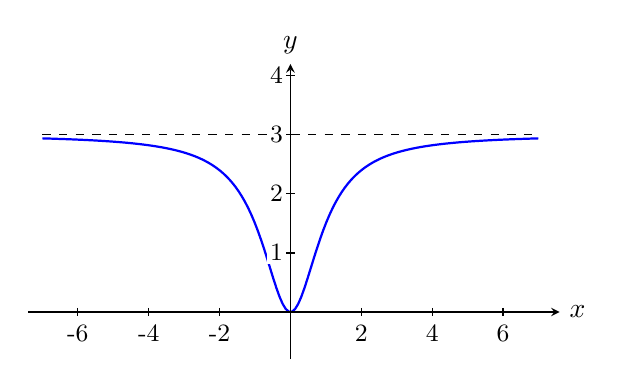
\begin{tikzpicture}[>=stealth, scale=0.75, x=0.6cm]
  % f(x) = 3x^2/(x^2 + 1): horizontal asymptote at y = 3
  \draw[blue, thick, samples=160, domain=-7:7] plot (\x, {3*\x*\x/(\x*\x+1)});
  % Horizontal asymptote
  \draw[dashed] (-7,3) -- (7,3);
  % Axes
  \draw[->] (-7.4,0) -- (7.6,0) node[right] {$x$};
  \draw[->] (0,-0.8) -- (0,4.2) node[above] {$y$};
  % x-axis ticks
  \foreach \x in {-6,-4,-2,2,4,6} {
    \draw (\x,0.07) -- (\x,-0.07) node[below, font=\small] {\x};
  }
  % y-axis ticks
  \foreach \y in {1,2,3,4} {
    \draw (0.12,\y) -- (-0.12,\y)
      node[left, font=\small, fill=white, inner sep=1pt] {\y};
  }
\end{tikzpicture}
\end{document}
